\documentclass[pdf,aspectratio=169]{beamer}
\usepackage[]{hyperref,graphicx,siunitx,booktabs,lmodern}
\usepackage{physics}
\usepackage{em-commands}
\mode<presentation>{\usetheme{EM}}

%Question Numbering
\newcounter{questionnumber}
\newcommand{\qnum}{%
	\stepcounter{questionnumber}%
	Q\arabic{questionnumber}
}
\resetcounteronoverlays{questionnumber}

\graphicspath{ {../Images/} }

\sisetup{per-mode=symbol}

\tikzstyle{plate}=[draw, very thick, minimum width=4cm, minimum height=1cm, fill=gray!40, anchor=south]

%preamble
\title{Its E-motional!}
\date{November 30, 2018}
\author{Jed Rembold}

\begin{document}
\renewcommand{\theenumi}{\Alph{enumi}}

\begin{frame}{Announcements}
	\begin{itemize}
		\item Homework
			\begin{itemize}
				\item Homework 12 is posted!
				\item 5 problems but generally I think more straightforward
				\item If you have it to me on time I'll do everything I can to have it graded by the last day of class.
			\end{itemize}
		\item Forgot to mention that I decided to give everyone an extra point on the Exam 2 since the in-class portion maybe ended up a smidgeon long.
		\item Still working on the grade reports, sorry. It's been a crazy week.
		\item I'll be giving blood or at the Senior talks the entire afternoon if you are trying to find me.
		\item Read the rest of 7.2 for Monday
	\end{itemize}
\end{frame}

\begin{frame}{\qnum}
	Still looking at the narrowing piece of our copper here. Assuming there is a steady current flowing through the copper what can you say about surface charge collecting on the sloped walls?
	\begin{center}
		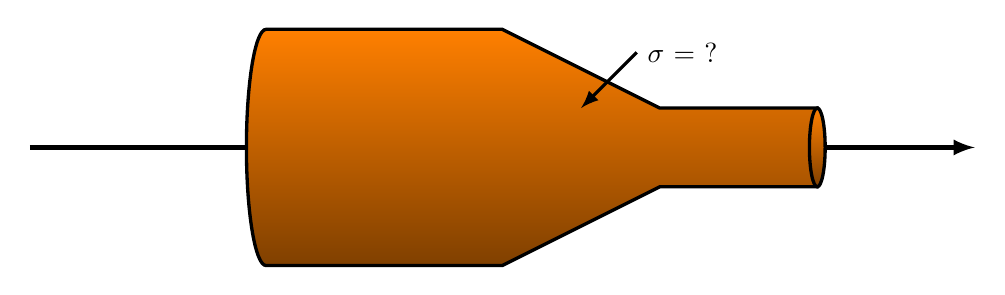
\begin{tikzpicture}
			\draw[ultra thick, -latex] (-6,0) -- (6,0);
			\draw[very thick, bottom color=orange!50!black, top color=orange]
				(4,0) -- ++(0,.5) -- ++(-2,0) -- ++(-2,1) -- ++(-3,0) arc(90:270:.25cm and 1.5cm)
				-- ++(3,0) -- ++(2,1) -- ++(2,0) -- cycle;
			\draw[very thick, bottom color=orange!50!black, top color=orange]
				(4,0) circle (.1cm and .5cm);
			\draw[latex-,very thick] (1,.5) -- +(45:1) node[right] {$\sigma$ = ?};
		\end{tikzpicture}
	\end{center}
	\begin{enumerate}
		\item No charge will accumulate
		\item \alert<2>{Positive charge will accumulate}
		\item Negative charge will accumulate
		\item Positive will accumulate on the top and negative on the bottom
	\end{enumerate}
\end{frame}

\begin{frame}{Demo for Surface Current}
	\begin{center}
		\includegraphics[width=0.4\textwidth]{SnakeyChargeDistribution.png}
	\end{center}
\end{frame}

\begin{frame}{\qnum}
	A circuit with an ideal battery is attached to a resistor. The force per charge inside the battery is
	\[\va{f} = \va{f}_{bat} + \ef\]
	and $A$ and $B$ are the locations of the two terminals of the battery.

	How many of the following statements are true?
	\begin{align*}
		\emf &= \oint \va{f}\vdot d\vell  &\emf &= \oint \va{f}_{bat}\vdot d\vell \\
		\emf &= \int_A^B \ef \vdot d\vell &\emf &= \int_A^B \va{f}_{bat}\vdot d\vell
	\end{align*}
	\begin{enumerate}
		\item 1
		\item 2
		\item \alert<2>{3}
		\item 4
	\end{enumerate}
\end{frame}

\begin{frame}{\qnum}
	Given that the emf is the line integral of the total force per unit charge around a closed loop, what are the units of the emf? (And can you prove it?)
	\begin{enumerate}
		\item Joules
		\item Amps
		\item Newtons
		\item \alert<2>{Volts}
	\end{enumerate}
\end{frame}

\begin{frame}{\qnum}
	A metal bar moves with a constant speed to the right. A constant magnetic field points into the page. What happens to the electrons in the bar (as seen in the frame of the moving bar)?
	\begin{enumerate}
		\item They move upward
		\item \alert<2>{They move downward}
		\item They move right
		\item Nothing
	\end{enumerate}
\end{frame}

\begin{frame}{\qnum}
	\begin{columns}
		\column{0.5\textwidth}
		One end of a rectangular metal loop enters a region of uniform magnetic field $\mf$ pointing out of the page. As the loop enters the field is there a non-zero emf around the loop?
		\begin{enumerate}
			\item \alert<2>{Yes, current will flow CW}
			\item Yes, current will flow CCW
			\item No
		\end{enumerate}
		
		
		\column{0.5\textwidth}
		\begin{center}
			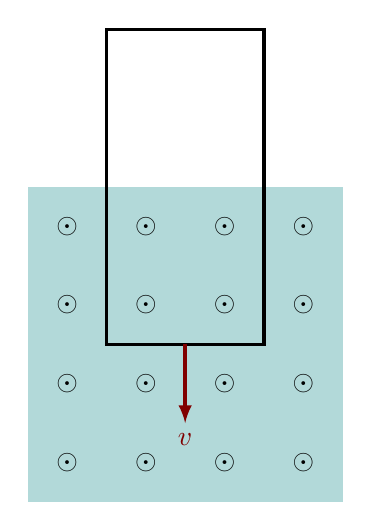
\begin{tikzpicture}
				\fill[Teal!30] (-2.5,-2.5) rectangle (1.5,1.5);
				\foreach \x in {-2,-1,0,1}{
					\foreach \y in {-2,-1,0,1}{
						\node at (\x,\y) {$\odot$};
					}
				}
				\draw[very thick] (-1.5,-.5) rectangle +(2,4);
				\draw[red!50!black, very thick, -latex] (-.5,-.5) -- +(0,-1) node[below] {$v$};
			\end{tikzpicture}
		\end{center}
	\end{columns}
\end{frame}

%\begin{frame}{\qnum}
	%A rectangular metal loop moves through the region of constant uniform magnetic field $\mf$ with speed $v$ at a particular time. What is the magnetic force on the \emph{loop} at this instant? You can assume the loop has some overall resistance $R$.
	%\begin{columns}
		%\column{0.5\textwidth}
		%\begin{center}
			%\begin{tikzpicture}
				%\fill[Teal!30] (-.5,-.5) rectangle (6.5,3.5);
				%\foreach \x in {0,1,...,6}{
					%\foreach \y in {0,1,...,3}{
						%\node at (\x,\y) {$\otimes$};
					%}
				%}
				%\draw[ultra thick] (.5,.5) rectangle +(3,2);
				%\draw[very thick, -latex, red!50!black] (3.5,1.5) -- +(1,0) node[right] {$v$};
				%\path[|<->|,thick]
					%(.3,.5) edge node[midway,left] {$h$} +(0,2)
					%(.5,2.7) edge node[pos=.33,above] {$w$} +(3,0);
			%\end{tikzpicture}
		%\end{center}
		%\column{0.5\textwidth}
		%\begin{enumerate}
			%\item 0
			%\item $\displaystyle \frac{vB^2 h^2}{R}$ to the left
			%\item $\displaystyle \frac{2vB^2 h^2}{R}$ to the left
			%\item $\displaystyle \frac{2vB^2 h^2}{R}$ to the right
		%\end{enumerate}
		
	%\end{columns}
%\end{frame}











\end{document}
